\iffalse
\documentclass[journal,12pt,twocolumn]{IEEEtran}
\usepackage{setspace}
\usepackage{gensymb}
\singlespacing
\usepackage[cmex10]{amsmath}
\usepackage{amsthm}
\usepackage{mathrsfs}
\usepackage{txfonts}
\usepackage{stfloats}
\usepackage{bm}
\usepackage{cite}
\usepackage{cases}
\usepackage{subfig}
\usepackage{longtable}
\usepackage{multirow}
\usepackage{enumitem}
\usepackage{mathtools}
\usepackage{steinmetz}
\usepackage{tikz}
\usepackage{circuitikz}
\usepackage{verbatim}
\usepackage{tfrupee}
\usepackage[breaklinks=true]{hyperref}
\usepackage{tkz-euclide}
\usetikzlibrary{calc,math}
\usepackage{listings}
    \usepackage{color}                                            %%
    \usepackage{array}                                            %%
    \usepackage{longtable}                                        %%
    \usepackage{calc}                                             %%
    \usepackage{multirow}                                         %%
    \usepackage{hhline}                                           %%
    \usepackage{ifthen}                                           %%
  %optionally (for landscape tables embedded in another document): %%
    \usepackage{lscape}     
\usepackage{multicol}
\usepackage{chngcntr}
\DeclareMathOperator*{\Res}{Res}
\renewcommand\thesection{\arabic{section}}
\renewcommand\thesubsection{\thesection.\arabic{subsection}}
\renewcommand\thesubsubsection{\thesubsection.\arabic{subsubsection}}

\renewcommand\thesectiondis{\arabic{section}}
\renewcommand\thesubsectiondis{\thesectiondis.\arabic{subsection}}
\renewcommand\thesubsubsectiondis{\thesubsectiondis.\arabic{subsubsection}}

% correct bad hyphenation here
\hyphenation{op-tical net-works semi-conduc-tor}
\def\inputGnumericTable{}                                 %%

\lstset{
frame=single, 
breaklines=true,
columns=fullflexible
}

\begin{document}


\newtheorem{theorem}{Theorem}[section]
\newtheorem{problem}{Problem}
\newtheorem{proposition}{Proposition}[section]
\newtheorem{lemma}{Lemma}[section]
\newtheorem{corollary}[theorem]{Corollary}
\newtheorem{example}{Example}[section]
\newtheorem{definition}[problem]{Definition}
\newcommand{\BEQA}{\begin{eqnarray}}
\newcommand{\EEQA}{\end{eqnarray}}
\newcommand{\define}{\stackrel{\triangle}{=}}

\bibliographystyle{IEEEtran}
\providecommand{\mbf}{\mathbf}
\providecommand{\pr}[1]{\ensuremath{\Pr\left(#1\right)}}
\providecommand{\qfunc}[1]{\ensuremath{Q\left(#1\right)}}
\providecommand{\sbrak}[1]{\ensuremath{{}\left[#1\right]}}
\providecommand{\lsbrak}[1]{\ensuremath{{}\left[#1\right.}}
\providecommand{\rsbrak}[1]{\ensuremath{{}\left.#1\right]}}
\providecommand{\brak}[1]{\ensuremath{\left(#1\right)}}
\providecommand{\lbrak}[1]{\ensuremath{\left(#1\right.}}
\providecommand{\rbrak}[1]{\ensuremath{\left.#1\right)}}
\providecommand{\cbrak}[1]{\ensuremath{\left\{#1\right\}}}
\providecommand{\lcbrak}[1]{\ensuremath{\left\{#1\right.}}
\providecommand{\rcbrak}[1]{\ensuremath{\left.#1\right\}}}
\theoremstyle{remark}
\newtheorem{rem}{Remark}
\newcommand{\sgn}{\mathop{\mathrm{sgn}}}
\providecommand{\abs}[1]{\left\vert#1\right\vert}
\providecommand{\res}[1]{\Res\displaylimits_{#1}} 
\providecommand{\norm}[1]{\left\lVert#1\right\rVert}
\providecommand{\mtx}[1]{\mathbf{#1}}
\providecommand{\mean}[1]{E\left[ #1 \right]}
\providecommand{\fourier}{\overset{\mathcal{F}}{ \rightleftharpoons}}
\providecommand{\system}{\overset{\mathcal{H}}{ \longleftrightarrow}}
\newcommand{\solution}{\noindent \textbf{Solution: }}
\newcommand{\cosec}{\,\text{cosec}\,}
\providecommand{\dec}[2]{\ensuremath{\overset{#1}{\underset{#2}{\gtrless}}}}
\newcommand{\myvec}[1]{\ensuremath{\begin{pmatrix}#1\end{pmatrix}}}
\newcommand{\mydet}[1]{\ensuremath{\begin{vmatrix}#1\end{vmatrix}}}
\numberwithin{equation}{subsection}
\makeatletter
\@addtoreset{figure}{problem}
\makeatother

\let\StandardTheFigure\thefigure
\let\vec\mathbf
\renewcommand{\thefigure}{\theproblem}



\def\putbox#1#2#3{\makebox[0in][l]{\makebox[#1][l]{}\raisebox{\baselineskip}[0in][0in]{\raisebox{#2}[0in][0in]{#3}}}}
     \def\rightbox#1{\makebox[0in][r]{#1}}
     \def\centbox#1{\makebox[0in]{#1}}
     \def\topbox#1{\raisebox{-\baselineskip}[0in][0in]{#1}}
     \def\midbox#1{\raisebox{-0.5\baselineskip}[0in][0in]{#1}}

\vspace{3cm}


\title{Assignment 1}
\author{Jaswanth Chowdary Madala}





% make the title area
\maketitle

\newpage

%\tableofcontents

\bigskip

\renewcommand{\thefigure}{\theenumi}
\renewcommand{\thetable}{\theenumi}


\begin{enumerate}

\textbf{Solution:}
\fi
The parameters used in the construction are shown in Table \ref{tab:chapters/9/10/6/9/1}.
Let the equations of these circles be given by
\begin{align}
\norm{\vec{x}}^2 + 2\vec{u_1}^\top\vec{x} + f &= 0 
\label{eq:chapters/9/10/6/9/1}\\
\norm{\vec{x}}^2 + 2\vec{u_2}^\top\vec{x} + f &= 0 
\label{eq:chapters/9/10/6/9/2}\\
\vec{u_1} = -\myvec{2\\0}, \, \vec{u_2} &= -\myvec{-2\\0}\\
f = -4. 
\end{align}
The common chord of the circles is given by
\begin{align}
2\vec{u_1}^\top\vec{x}-2\vec{u_2}^\top\vec{x}+f_1 - f_2 &= 0\\
\implies
\myvec{1&0}\vec{x} &= 0
\label{eq:chapters/9/10/6/9/3}
\end{align}
\eqref{eq:chapters/9/10/6/9/3} can be written in parametric form as
\begin{align}
	\vec{h} &= \myvec{0\\0}, \, \vec{m} = \myvec{0\\1}\\
	\vec{x} &= \vec{h}+ \mu \vec{m}
\label{eq:chapters/9/10/6/9/4}
\end{align} 
The parameter $\mu$ for the points of intersection of the above line with the given conic
		%line \eqref{eq:chapters/9/10/6/9/5} with the conic section \eqref{eq:chapters/9/10/6/9/6}
is given by the equation 
\begin{align}
\mu^2\vec{m}^{\top}\vec{V}\vec{m} + 2 \mu\vec{m}^{\top}\brak{\vec{V}\vec{h}+\vec{u}} + \text{g}\brak{\vec{h}} &=0
\label{eq:chapters/9/10/6/9/7}
\end{align}
Substituting numerical values,
\begin{align}
\vec{V} = \vec{I}, \, \vec{u} &= \myvec{-2\\0}, \, f = -4,\,
\vec{h} = \myvec{0\\0}, \, \vec{m} &= \myvec{0\\1}\\
\end{align}
we obtain 
\begin{align}
\mu^2 - 4 =0
\implies \mu = \pm 2
\end{align}
From \eqref{eq:chapters/9/10/6/9/4}, 
\begin{align}
\vec{A} = \myvec{0\\2},\,
\vec{B} = \myvec{0\\-2} 
\end{align} 
Since 
\begin{align}
\vec{m} = \myvec{2\\1}
\label{eq:chapters/9/10/6/9/8}
\end{align} 
The equation of the line passing through the point $\vec{A}$ with the direction vector \eqref{eq:chapters/9/10/6/9/8} in parametric form is given by,
\begin{align}
\vec{x} = \myvec{0\\2} + \alpha\myvec{2\\1}
\label{eq:chapters/9/10/6/9/9}
\end{align}
Substituing 
\begin{align}
\vec{V} = \vec{I}, \, \vec{u} &= \myvec{-2\\0}, \, f = -4
\vec{h} = \myvec{0\\2}, 
\end{align}
the intersection of the line in 
\ref{eq:chapters/9/10/6/9/9}
with one circle is given by 
\begin{align}
5\alpha^2 - 4 \alpha &=0
\implies \alpha &= 0, \frac{4}{5}
\end{align}
Thus,
\begin{align}
\vec{P} &= \myvec{\frac{8}{5}\\\\ \frac{14}{5}}
\end{align}
Similarly, the intersection with the second circle is given by 
\begin{align}
	5\beta^2 + 12 \beta &=0,\,
\implies \beta = 0, -\frac{12}{5}\\
	\text{and } \vec{Q} &= \myvec{-\frac{24}{5}\\\\-\frac{2}{5}}
\end{align}
Thus, 
\begin{align}
	\norm{\vec{B}-\vec{P}} &=  
\norm{\vec{B}-\vec{Q}} =  \frac{8\sqrt{10}}{5}
\\
\implies 
	BP &= BQ.
\end{align}
See Fig.
\ref{fig:chapters/9/10/6/9/1}.
\begin{table}[H]
\centering
\begin{tabular}{|p{3cm}|p{3cm}|p{3cm}|}
\hline                                        
\textbf{Symbol} & \textbf{Values} & \textbf{Description}\\                                          
\hline                                 
$\theta$ & 30$\degree{}$   & $\angle{BAD} = \angle{BAC}$ \\           
\hline                                    
a &  9 & $AB$ \\     
\hline                      
c & 5 & $AC$ \\
\hline                                     
		$\vec{e}_1$ & $\myvec{
			1\\
			0\\
			}$ & basis vector\\ 
\hline
\end{tabular}

\caption{}
\label{tab:chapters/9/10/6/9/1}
\end{table}
\begin{figure}[H]
\centering
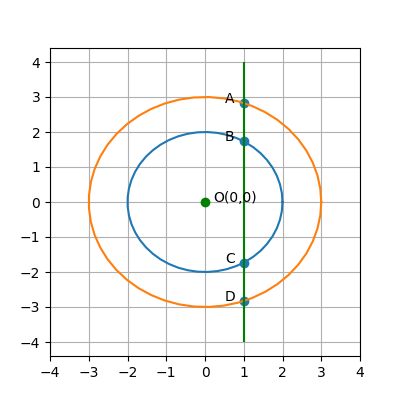
\includegraphics[width=0.75\columnwidth]{chapters/9/10/6/9/figs/fig.png}
\caption{}
\label{fig:chapters/9/10/6/9/1}
\end{figure}
